% \setchapterpreamble[u]{\margintoc}
% \chapter{Margin Stuff}

% Sidenotes are a distinctive feature of all 1.5-column-layout books.
% Indeed, having wide margins means that some material can be displayed
% there. We use margins for all kind of stuff: sidenotes, marginnotes,
% small tables of contents, citations, and, why not?, special boxes and
% environments.

% \section{Sidenotes}

% Sidenotes are like footnotes, except that they go in the margin, where
% they are more readable. To insert a sidenote, just use the command
% \Command{sidenote\{Text of the note\}}. You can specify a
% mark\sidenote[O]{This sidenote has a special mark, a big O!} with \\
% \Command{sidenote[mark]\{Text\}}, but you can also specify an offset,
% which moves the sidenote upwards or downwards, so that the full syntax is:

% \begin{lstlisting}[style=kaolstplain]
% \sidenote[mark][offset]{Text}
% \end{lstlisting}

% If you use an offset, you always have to add the brackets for the mark,
% but they can be empty.\sidenote{If you want to know more about the usage
% of the \Command{sidenote} command, read the documentation of the
% \Package{sidenotes} package.}

% In \Class{kaobook} we copied a feature from the \Package{snotez}
% package: the possibility to specify a multiple of \Command{baselineskip}
% as an offset. For example, if you want to enter a sidenote with the
% normal mark and move it upwards one line, type:

% \begin{lstlisting}[style=kaolstplain]
% \sidenote[][*-1]{Text of the sidenote.}
% \end{lstlisting}

% As we said, sidenotes are handled through the \Package{sidenotes}
% package, which in turn relies on the \Package{marginnote} package.

% \section{Marginnotes}

% This command is very similar to the previous one. You can create a
% marginnote with \Command{marginnote[offset]\{Text\}}, where the offset
% argument can be left out, or it can be a multiple of
% \Command{baselineskip},\marginnote[-1cm]{While the command for margin
% notes comes from the \Package{marginnote} package, it has been redefined
% in order to change the position of the optional offset argument, which
% now precedes the text of the note, whereas in the original version it
% was at the end. We have also added the possibility to use a multiple of
% \Command{baselineskip} as offset. These things were made only to make
% everything more consistent, so that you have to remember less things!}
% \eg

% \begin{lstlisting}[style=kaolstplain]
% \marginnote[-12pt]{Text} or \marginnote[*-3]{Text}
% \end{lstlisting}

% \begin{kaobox}[frametitle=To Do]
% A small thing that needs to be done is to renew the \Command{sidenote}
% command so that it takes only one optional argument, the offset. The
% special mark argument can go somewhere else. In other words, we want the
% syntax of \Command{sidenote} to resemble that of \Command{marginnote}.
% \end{kaobox}

% We load the packages \Package{marginnote}, \Package{marginfix} and
% \Package{placeins}. Since \Package{sidenotes} uses \Package{marginnote},
% what we said for marginnotes is also valid for sidenotes. Side- and
% margin- notes are shifted slightly upwards
% (\Command{renewcommand\{\textbackslash marginnotevadjust\}\{3pt\}}) in
% order to align them to the bottom of the line of text where the note is
% issued. Importantly, both sidenotes and marginnotes are defined as
% floating if the optional argument (\ie the vertical offset) is left
% blank, but if the offset is specified they are not floating. Recall that
% floats cannot be nested, so in some rare cases you may encounter errors
% about lost floats; in those cases, remember that sidenotes and
% marginnotes are floats. To solve the problem, it may be possible to
% transform them into non-floating elements by specifying an offset of
% 0pt.

% \section{Footnotes}

% Even though they are not displayed in the margin, we will discuss about
% footnotes here, since sidenotes are mainly intended to be a replacement
% of them. Footnotes force the reader to constantly move from one area of
% the page to the other. Arguably, marginnotes solve this issue, so you
% should not use footnotes. Nevertheless, for completeness, we have left
% the standard command \Command{footnote}, just in case you want to put a
% footnote once in a while.\footnote{And this is how they look like.
% Notice that in the PDF file there is a back reference to the text;
% pretty cool, uh?}

% \section{Margintoc}

% Since we are talking about margins, we introduce here the
% \Command{margintoc} command, which allows one to put small table of
% contents in the margin. Like other commands we have discussed,
% \Command{margintoc} accepts a parameter for the vertical offset, like
% so: \Command{margintoc[offset]}.

% The command can be used in any point of the document, but we think it
% makes sense to use it just at the beginning of chapters or parts. In
% this document I make use of a \KOMAScript\xspace feature and put it in
% the chapter preamble, with the following code:

% \marginnote{The font used in the margintoc is the same as the one for
% 	the chapter entries in the main table of contents at the beginning
% 	of the document.}

% \begin{lstlisting}[style=kaolstplain]
% \setchapterpreamble[u]{\margintoc}
% \chapter{Chapter title}
% \end{lstlisting}

% As the space in the margin is a valuable resource, there is the
% possibility to print a shorter version of the title in the margin toc.
% Thus, there are in total three possible versions for the title of a
% section (or subsection): the one for the main text, the one for the main
% table of contents, and the one for the margintoc. These versions can be
% specified at the same time when the section is created in the source
% \TeX file:
% \begin{lstlisting}[style=kaolstplain]
% \section[alternative-title-for-toc]{title-as-written-in-text}[alternative-title-for-margintoc]
% \end{lstlisting}

% By default, the margintoc includes sections and subsections.
% If you only want to show sections, add
% \begin{lstlisting}[style=kaolstplain]
% \setcounter{margintocdepth}{\sectiontocdepth}
% \end{lstlisting}
% somewhere in your preamble.

% \section{Marginlisting}

% On some occasions it may happen that you have a very short piece of code
% that doesn't look good in the body of the text because it breaks the
% flow of narration: for that occasions, you can use a
% \Environment{marginlisting}. The support for this feature is still
% limited, especially for the captions, but you can try the following
% code:

% \begin{marginlisting}[-1.35cm]
% 	\caption{An example of a margin listing.}
% 	\vspace{0.6cm}
% 	\begin{lstlisting}[language=Python,style=kaolstplain]
% print("Hello World!")
% 	\end{lstlisting}
% \end{marginlisting}

% \begin{verbatim}
% \begin{marginlisting}[-0.5cm]
% 	\caption{My caption}
% 	\vspace{0.2cm}
% 	\begin{lstlisting}[language=Python,style=kaolstplain]
% 	... code ...
% 	\end{lstlisting}
% \end{marginlisting}
% \end{verbatim}

% Unfortunately, the space between the caption and the listing must be
% adjusted manually; if you find a better way, please let me know.

% Not only textual stuff can be displayed in the margin, but also figures.
% Those will be the focus of the next chapter.

\setchapterpreamble[u]{\margintoc}
\chapter{Delta function potential}

We want to understand solids and their properties, for example why copper is a conductor and wood is not? For this and other questions we will propose our next problem, the delta function potential problem.


\section{Definition of the potential}

We define our potential this time as

\begin{equation}
    \label{4.1}
    V(x) = -2C\delta(x)
\end{equation}

Where $C= V_0a$.

\begin{marginfigure}
  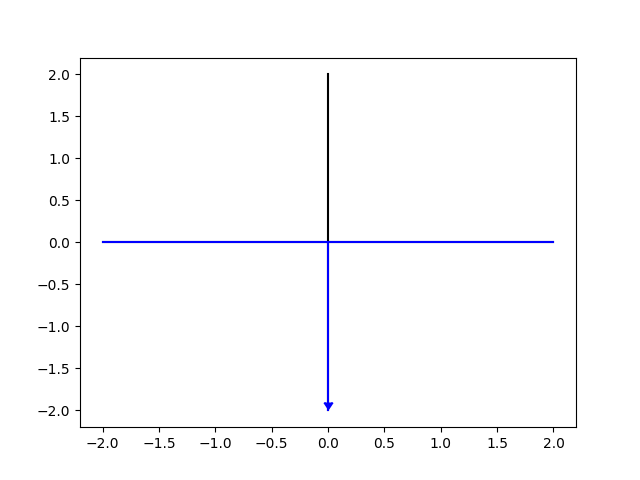
\includegraphics{images4/delta.png}
  \caption{Delta function potential}
  \label{figure4-1}
\end{marginfigure}

Because we have delta functions in our equations we can not call them normal equations so we will use quotes to differentiate them from real equations.

\begin{equation}
    "+\frac{\hbar^2}{2m}\frac{\partial^2\phi}{\partial x^2} + 2C\delta(x) \phi(x) = + E \phi(x)"
\end{equation}

\section{Solution}

The solution for this equation is:

\begin{equation}
    \label{4.3}
    \psi(x,t) = e^{i\frac{E}{\hbar}t} \phi(x)
\end{equation}

Now we need to solve our equation for $\phi(x)$.

\begin{equation}
    \label{4.4}
    \begin{split}
    & "\frac{\partial^2\phi}{\partial x^2}+\frac{4mC}{\hbar^2}\delta(x)\phi(x)= \frac{2mE}{\hbar^2}\phi(x)" \\
    & "\frac{\partial^2\phi}{\partial x^2}+\frac{4mV_0a}{\hbar^2}\delta(x)\phi(x)= \frac{2mE}{\hbar^2}\phi(x)"
    \end{split}
\end{equation}

We need to define two variables to resolve this equations, $\alpha$ and g (This variables are completely different to the variables in the previous chapter).

\begin{equation}
    \label{4.5}
    \begin{split}
    & g = \frac{2mV_0a}{\hbar^2} \\
    & \alpha = \sqrt{\frac{2mE}{\hbar^2}}
    \end{split}
\end{equation}

As we did in the previous chapter we have to think about the continuity in $\phi(x)$. Can $\phi(x)$ be discontinuous? The answer is no. $\phi(x)$ is continuous because if it weren't continues the second derivative would look like the derivative of a delta function and the equations don't make sense with that assumption. However, in this case the first derivative of $\phi(x)$ must be discontinuous because we need the second derivative to go as a delta function.

We solve for $\phi(x) \neq 0$.

\begin{equation}
    \label{4.6}
    \frac{\partial^2\phi(x)}{\partial x^2} = \alpha^2\phi(x)
\end{equation}

The solution to this differential equation is:

\begin{equation}
    \label{4.7}
    \begin{split}
        \phi(x)= \left\{ \begin{array}{lcc} Ae^{\alpha x} & where & x \leq 0 \\
        \\ Ae^{-\alpha x} & where & x \geq 0 \end{array} \right.
    \end{split}
\end{equation}

And the derivatives are going to be:

\begin{equation}
    \label{4.8}
        \frac{\partial\phi(x)}{\partial x}= \left\{ \begin{array}{lcc} A\alpha e^{\alpha x} & where & x \leq 0 \\
        \\ -A\alpha e^{-\alpha x} & where & x \geq 0 \end{array} \right.
\end{equation}

\begin{equation}
    \label{4.9}
        "\frac{\partial^2\phi(x)}{\partial x^2}= \left\{ \begin{array}{lcc} A\alpha^2 e^{\alpha x} & where & x \leq 0 \\
        \\ A\alpha^2 e^{-\alpha x} & where & x \geq 0 \end{array} \right. +B\delta(x)"
\end{equation}

To solve for A we are going to use the continuity conditions we mention before and the fundamental theorem of calculus.

\begin{equation}
    \label{4.10}
        \begin{array}{c}
            \int_{-\infty}^{\infty} \frac{\partial^2\phi(x)}{\partial x^2} dx = \left[ \frac{\partial \phi}{\partial x}\right]_{x=-\infty} - \left[ \frac{\partial \phi}{\partial x}\right]_{x=\infty}
            \\

            \\
            A\alpha^2\int_{-\infty}^{0}e^{\alpha x}dx+ A \alpha^2\int_{0}^{\infty}e^{-\alpha x}dx+B\int_{-\infty}^{-\infty}\delta(x) dx = 0
            \\

            \\
            A\alpha+A\alpha +B = 0
            \\

            \\
            B = -2A\alpha
        \end{array}
\end{equation}

We want to integrate \ref{4.4} for x=0 to remove the quotes.

\begin{equation}
    \label{4.11}
        \begin{array}{c}
            A\alpha^2\int_{-\infty}^{0}e^{\alpha x}dx+ A \alpha^2\int_{0}^{\infty}e^{-\alpha x}dx+ = \int_{-\infty}^{\infty} \frac{\partial^2\phi(x)}{\partial x^2} dx + 2g\int_{-\infty}^{\infty}\delta(x)\phi(x)dx
            \\

            \\
            \left[\alpha Ae^{\alpha x}\right]_{-\infty}^{0}-\left[\alpha Ae^{\alpha x}\right]_{0}^{\infty} = 0 + 2g\phi(0)
            \\

            \\
            2\alpha A = 2gA
            \\

            \\
            \alpha = g
        \end{array}
\end{equation}

In this case we only have one possible value for $\alpha$ so only one Energy level is possible. The solution to the problem is:

\begin{equation}
\label{4.12}
\phi(x) = \left\{ \begin{array}{lcc}
     Ae^{gx}    & where  &  x<0  \\
     Ae^{-gx}   & where  &  x<0
\end{array}\right.
\end{equation}

\begin{equation}
\label{4.13}
P(x) = \left\{ \begin{array}{lcc}
     A^2e^{2gx}    & where  &  x<0  \\
     A^2e^{-2gx}   & where  &  x<0
\end{array}\right.
\end{equation}

\begin{figure}
  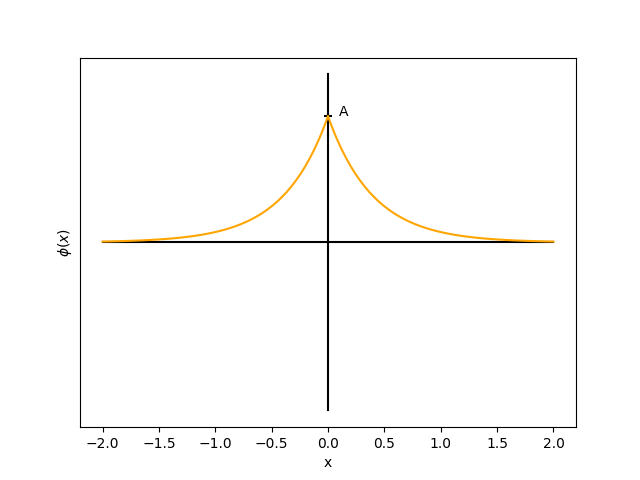
\includegraphics{images4/phi(x).png}
  \centering
  \caption{Solution for g=2.5 of phi(x) for the delta function potential.}
  \labfig{figure4-2}
\end{figure}


To solve for A we need to use the property from \ref{3.3}.

\begin{equation}
\label{4.14}
P(x) = \left\{ \begin{array}{lcc}
     A^2e^{2gx}    & where  &  x<0  \\
     A^2e^{-2gx}   & where  &  x<0
\end{array}\right.
\end{equation}

\begin{equation}
\label{4.15}
\begin{array}{c}
     \int_{-\infty}^{\infty}P(x) dx = 1
     \\

     \\
     \frac{A^2}{g}=1
     \\

     \\
     A^2 = g
\end{array}
\end{equation}

We have finally solved the problem and the solution is:

\begin{equation}
\label{4.16}
\phi(x) = \left\{ \begin{array}{lcc}
     \sqrt{g}e^{gx}    & where  &  x<0  \\
     \sqrt{g}e^{-gx}   & where  &  x<0
\end{array}\right.
\end{equation}

We will not do examples using this model because is not that usefull, but it will help us understand the next problem better.

